% !TeX spellcheck = ru_RU
% !TEX root = vkr.tex

\section{Обзор}
\label{sec:relatedworks}

В данном разделе представлен обзор модели Голланда и дано краткое описание психометрических тестов личности. Проведен обзор предметной области: рассмотрены и проанализированы статьи, предлагающие различные подходы к решению задачи предсказания значений факторов психометрических тестов и нахождения взаимосвязей между факторами.

\subsection{Модель Голланда и психометрические тесты личности}
\subsubsection{Модель Голланда RIASEC}

Одним из основных инструментов оценки профессиональных интересов служит модель Голланда, также известная как модель \textit{RIASEC}. Данная методика была разработана Джоном Льюисом Голландом в конце 1950-х годов~\cite{Holland1959}, после чего им неоднократно дорабатывалась и развивалась. В своей статье \enquote{Теория профессионального выбора} исследователь сопоставляет различным типам личности профессиональные роды деятельности. Согласно Голланду, личности выбирают и преуспевают в той профессиональной среде, которая подходит их характеру, является отражением их базовых черт, при этом профессиональная карьерная среда классифицируется по тем типам личностей, которые в этой среде успешны. Таким образом, для определения профессиональных предпочтений достаточно определить социально-профессиональный тип личности.

В своих более поздних работах ученый выделяет следующие шесть типов личностей:
\begin{itemize}[noitemsep, topsep=0pt, parsep=0pt, partopsep=0pt]
  \item реалистический (\textit{Realistic}, R);
  \item исследовательский (\textit{Investigative}, I);
  \item артистический (\textit{Artistic}, A);
  \item социальный (\textit{Social}, S);
  \item предприимчивый (\textit{Enterprising}, E);
  \item традиционный (\textit{Conventional}, C).
\end{itemize}

При этом определяется не единственный тип личности: оценивается принадлежность человека к каждому из типов, которые затем выстраиваются в порядке убывания их выраженности. Результат записывается в виде кода по первым буквам типов, что и дало название модели. Модель Голланда также можно представить как правильный шестиугольник с кодами в вершинах (рисунок~\ref{fig:hexagon_RIASEC}).

\begin{figure}
    \centering
    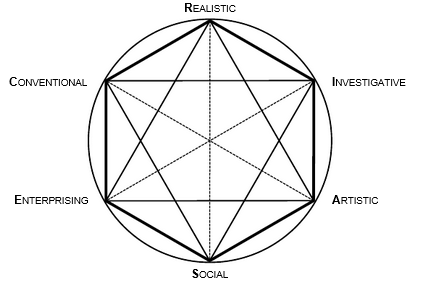
\includegraphics[width=0.65\linewidth]{figures/hexagon_RIASEC.png}
    \caption{Правильный шестиугольник, в вершинах которого расположены типы личности (коды) согласно Голланду\protect\footnotemark}
    \label{fig:hexagon_RIASEC}
\end{figure}

\footnotetext{Источник: Hexagonal arrangement of the RIASEC dimensions. URL: \url{https://www.researchgate.net/figure/Hexagonal-arrangement-of-the-RIASEC-dimensions_fig1_356677137}}

Существуют различные методики определения кода Голланда, и в российской адаптации методики Г.~В.~Резапкиной~\cite{Rezapkina} предлагается опросный инструмент с 42 парами профессий: из каждой пары опрашиваемый должен выбрать одну профессию, которая его более привлекает. Каждой из выбранных профессий сопоставляется один из шести типов, соответствие профессий и типов было произведено Голландом в своих работах и дополнено другими исследователями. Для каждого из типов подсчитывается количество упоминаний, и шесть типов выстраиваются в порядке убывания подсчитанных баллов. Например, опрашиваемый 11 раз в парах выбрал профессии, соответствующие исследовательскому типу (I), 10~--- традиционному (C), 9, 7, 5 и 0 предприимчивому (E), реалистическому (R), социальному (S) и артистическому (A) типам соответственно. Итоговым кодом для опрашиваемого будет \enquote{ICERSA}, который можно ограничить тремя первыми буквами (\enquote{верхняя триада}, \enquote{ICE}).

\label{subsec:cindex}
Для сравнения кода типа личности и кода его профессиональной среды Голланд вводит понятие конгруэнтности (согласованности). Среди мер согласованности можно выделить C‑индекс для трёхбуквенных кодов (\enquote{верхних триад}):
  \[
    C = 3\, (X_1, Y_1) + 2\, (X_2, Y_2) + 1\, (X_3, Y_3),
  \]
  где $\{X_i\}$ и $\{Y_i\}$ — первые три позиции кодов Голланда, их позиции в замкнутой цепочке (шестиугольнике) \textit{R-I-A-S-E-C}:
  \[
    (X_i, Y_i) =
    \begin{cases}
      3, & \text{если $X_i = Y_i$,}\\
      2, & \text{если $X_i$ и $Y_i$ -- соседние позиции,}\\
      1, & \text{если $X_i$ и $Y_i$ -- позиции через один код,}\\
      0, & \text{если $X_i$ и $Y_i$ -- противоположны.}
    \end{cases}
  \]
Б\'oльшие значения меры согласованности говорят о большем сходстве двух профессиональных профилей (кодов Голланда). 


\subsubsection{Психометрические тесты личности}
\label{sec:psytests}

Помимо модели Голланда есть и другие способы определения проф\-ори\-ента\-цион\-ных предпочтений. Одним из таких способов являются пси\-хо\-мет\-ри\-чес\-кие опросные инструменты. Их основная цель~--- отразить некоторые черты личности человека в удобном числовом формате. Они помогают выявить ключевые черты характера, тем\-пе\-ра\-мент, цен\-ности и по\-ве\-ден\-ческие особенности. 

Среди психометрических тестов личности можно выделить следующие (в скобках указано количество факторов):
    \begin{enumerate}[noitemsep, topsep=0pt, parsep=0pt, partopsep=0pt]
        \item Опросник Леонгарда-Шмишека (10).
        \item Личностный опросник Айзенка (4).
        \item 16-факторный опросник Кеттелла (16).
        \item Пятифакторный опросник личности (\enquote{Большая пятёрка}; 5).
        \item Ценностный опросник Шварца (20).
    \end{enumerate}

Опросник Леонгарда-Шмишека разработан Г.~Шмишеком на основе теории акцентуаций личности К.~Леонгарда~\cite{Schmieschek} (адаптация на русский язык~--- ~\cite{Kortneva}) и представляет собой опросник из 88 вопросов с ответами \enquote{да/нет}. Вопросы сгруппированы по 10 шкалам, по каждой из которых подсчитывается балл, отражающий выраженность соответствующей акцентуации. Методика позволяет составить индивидуальный психологический портрет, выявить усиленные черты характера, влияющие на поведение, эмоциональные реакции и адаптацию. Применяется в образовательных программах, при подборе персонала и профориентации.

Личностный опросник Айзенка (EPQ-R) разработан Г.~Айзенком и коллегами в 1985~г.~\cite{Eysenck} (русская адаптация Суходольского~\cite{Sukhodolsky}) и направлен на измерение базовых личностных параметров: экстраверсии, нейротизма, психотизма и оценки искренности ответов. Опросник включает 100 вопросов с ответами \enquote{да/нет}, по результатам которых формируются соответствующие шкалы, позволяющие оценить стиль взаимодействия человека с окружающим миром, его стрес\-со\-ус\-той\-чивость и темперамент. Методика широко применяется в клинической психологии, образовательных программах, профориентации и научных исследованиях.

16-факторный опросник Кеттелла (16PF)~\cite{Cattell} (адаптация~\cite{Shmelev}) предназначен для всесторонней диагностики личности через измерение 16 основных черт характера методом факторного анализа. Тест состоит из 187 вопросов с ответами \enquote{утвердительно}, \enquote{отрицательно} и \enquote{нейтрально}, что позволяет получить детальный личностный профиль. По итогам подсчитываются баллы по каждой из 16 шкал (от 0 до 26) и дополнительным шкалам, отражающим вторичные личностные особенности. Инструмент широко применяется при кадровом отборе, психологическом консультировании и научных исследованиях для глубокого понимания индивидуальных различий. Именно 16PF послужил основой для появления пятифакторных тестов (\enquote{Большая пятёрка}).

Пятифакторный опросник личности (\enquote{Большая пятёрка}, 5PFQ)~\cite{Tsuji} (русская адаптация Хромова~\cite{Khromov}) основан на модели факторного анализа \textit{NEO-PI-R}~\cite{Costa} и представляет собой диспозиционную методику для оценки пяти базовых черт личности: экстраверсия, привязанность, самоконтроль, эмоциональная устойчивость, экспрессивность. Тест включает 75 утверждений, которые оцениваются от –2 до 2, что позволяет получить итоговые шкалы, отражающие степень выраженности каждой черты, а также множество вторичных факторов. Инструмент широко применяется в профориентации, подборе персонала и научных исследованиях.

Ценностный опросник Шварца (SVS)~\cite{Schwartz} (русская адаптация Карандашева~\cite{Karandashev}) предназначен для количественной оценки 10 универсальных ценностей, выявленных методом исследования жизненных приоритетов. Методика использует парное сравнение ценностей и фиксирует две оценки: нормативный идеал (какие ценности человек считает важными в идеале) и индивидуальный приоритет (что важно для него лично). Опросник активно применяется в социологических и психологических исследованиях для анализа культурных различий и индивидуальных мотивационных профилей.


\subsection{Методы машинного обучения в вычислительной психологии личности}

Применению методов машинного обучения в вычислительной психологии личности (\emph{personality computing}) в целом и нахождению взаимосвязей результатов различных психометрических тестов между собой в частности посвящено множество научных работ. Для решения задачи установления взаимосвязи между факторами психологических тестов, а также внешними признаками используются следующие методы:

\begin{itemize}[noitemsep, topsep=0pt, parsep=0pt, partopsep=0pt]
  \item Статистические: регрессионный, корреляционный, факторный анализ; структурное моделирование (\emph{SEM}).
  \item Динамические: модели, описывающие изменения во времени (дифференциальные уравнения).
  \item Сетевые: анализ взаимосвязей между переменными как узлов в сети.
  \item Машинное обучение: классификация, кластеризация, регрессия, ранжирование.
\end{itemize}

Так, всё чаще встречается применение методов машинного обучения в вычислительной психологии. Задачи могут быть различны.
\begin{itemize}
    \item Предсказание кода Голланда на основе социально-демо\-графических признаков~\cite{Bogacheva}. Авторы предлагают различные подходы для решения этой задачи: с тех пор как код Голланда может быть представлен и как последовательно идущие три или шесть кодов, и как целочисленные значения кодов, то и задача может быть поставлена следующим образом: регрессия с множественными выходами (\textit{многоцелевая}; \emph{multi\-output regression}), классификация с несколькими метками (\emph{multi\-label classification}), классификация с множественными выходами (\emph{multi\-output classification}). Авторы отмечают: в случае последовательного предсказания для многоцелевой регрессии порядок предсказания выходов важен. В качестве меры сходства авторы используют меру конгруэнтности~--- C-индекс. Наилучшие результаты показал градиентный бустинг: $\text{C‑index} = 10.95$ при решении задачи регрессии и $\text{C‑index} = 11.08$ при решении задачи классификации.
    
    \item Оценка профессионального выбора~\cite{Song}. Пользователю по результатам прохождения теста Голланда предъявлялся список профессий, которым прежде уже был сопоставлен свой код Голланда; требовалось найти наиболее подходящие профессии. Наилучших результатов удалось достичь с помощью комбинации традиционных методов и ансамбля методов машинного обучения. В качестве традиционных методов использовалось сравнение значений мер конгруэнтности (простое совпадение главного фактора кода Голланда, оценка профилей~--- числовых значений кода Голланда~--- с помощью таких метрик, как коэффициент корреляции Пирсона и Евклидово расстояние). В ансамбль методов машинного обучения вошли следующие модели: многослойный перцептрон (нейронная сеть), метод k-ближайших соседей, регуляризованная регрессия, случайный лес.
    
    \item В статье~\cite{Usslepp} применяется логистическая регрессия для предсказания (классификации), какой путь выберут учащиеся: академический или профессиональный; предикторами служили значения факторов тестов Голланда и \enquote{Большой пятерки}.
    
    \item Расширение списка профессий, поставленных в соответствие кодам Голланда, путем создания платформы для автоматизации профилирования вакансий~\cite{Silva}. Предсказание кодов Голланда решается как задача ранжирования с метрикой NDCG (\textit{Normalized Discounted Cumulative Gain}).
    
    \item Предсказание значений шкал теста \enquote{Большой пятерки} пользователей социальных сетей по следующим признакам: их посты, комментарии, репосты и численные характеристики аккаунта пользователя. Решалась задача бинарной классификации (шкалы теста были представлены бинарными путем сравнения с пороговым значением) с использованием моделей случайного леса и метода опорных векторов~\cite{Stankevich}. Подобная задача в работе~\cite{Basaran} решалась с помощью многослойного перцептрона. По схожим признакам (в т.~ч. по указанной в профиле пользователя информации) для оценки темперамента (тест Айзенка EPQ) в статье~\cite{Oliseenko} использовались модели CatBoost и случайный лес. В работе~\cite{Titov} предсказание результатов тестов \enquote{Большой пятерки}, Шварца и других по извлекаемым из профилей в социальной сети численным признакам (число друзей, постов, подписок, длина поля с личным описанием, длина постов и др.) осуществляется с помощью модели XGBoost (\emph{eXtreme Gradient Boosting}).
\end{itemize}

\subsection{Выводы}

Для предсказания кода Голланда могут быть использованы различные идеи, рассмотренные в данном обзоре. Например, задачу можно сформулировать как регрессию/классификацию с множественными выходами (\emph{multioutput}), классификацию с несколькими метками (\emph{multilabel}). Для многоцелевой регрессии могут быть использованы различные метрики: не только усредненные MSE или RMSE, часто применяемые в таких задачах, но и специальные меры конгруэнтности (\textit{сходства}, C-индекс), косинусное расстояние, коэффициент корреляции. Приведены различные методы машинного обучения, в том числе и те, с помощью которых были достигнуты наилучшие результаты: в первую очередь, это градиентный бустинг (CatBoost, XGBoost) и случайный лес. В соответствии с результатами работы~\cite{Bogacheva} приемлемым может считаться следующий результат предсказания значений кода Голланда: $\text{C‑index} \geq 11$.

Несмотря на разнообразие работ, наличие среди них тех, где по результатам одних психометрических тестов предсказываются другие, до сих пор нет инструментов, позволяющих по результатам сразу нескольких популярных психометрических тестов~--- \enquote{Большой пятерки}, Кеттелла, Айзенка, Леонгарда, Шварца~--- предсказать код Голланда. Таким образом, пользователь мог бы получить информацию о своих профориентационных предпочтениях без прохождения теста Голланда. Кроме того, даже при прохождении последнего подобный инструмент мог бы уточнять результаты теста Голланда, проверять его непротиворечивость в соответствии с результатами других тестов.
